\documentclass{article}

\usepackage{graphicx}
\usepackage{tikz}
\usepackage{tikzsymbols}
\usetikzlibrary{calc,patterns,shapes.geometric}
\pagestyle{empty}
\usepackage[margin=0pt]{geometry}
\geometry{papersize={14in,12in}}

\def\centerarc[#1](#2)(#3:#4:#5){\draw[#1] ($(#2)+({#5*cos(#3)},{#5*sin(#3)})$) arc (#3:#4:#5);}

\begin{document}
	\begin{figure}
		\centering
		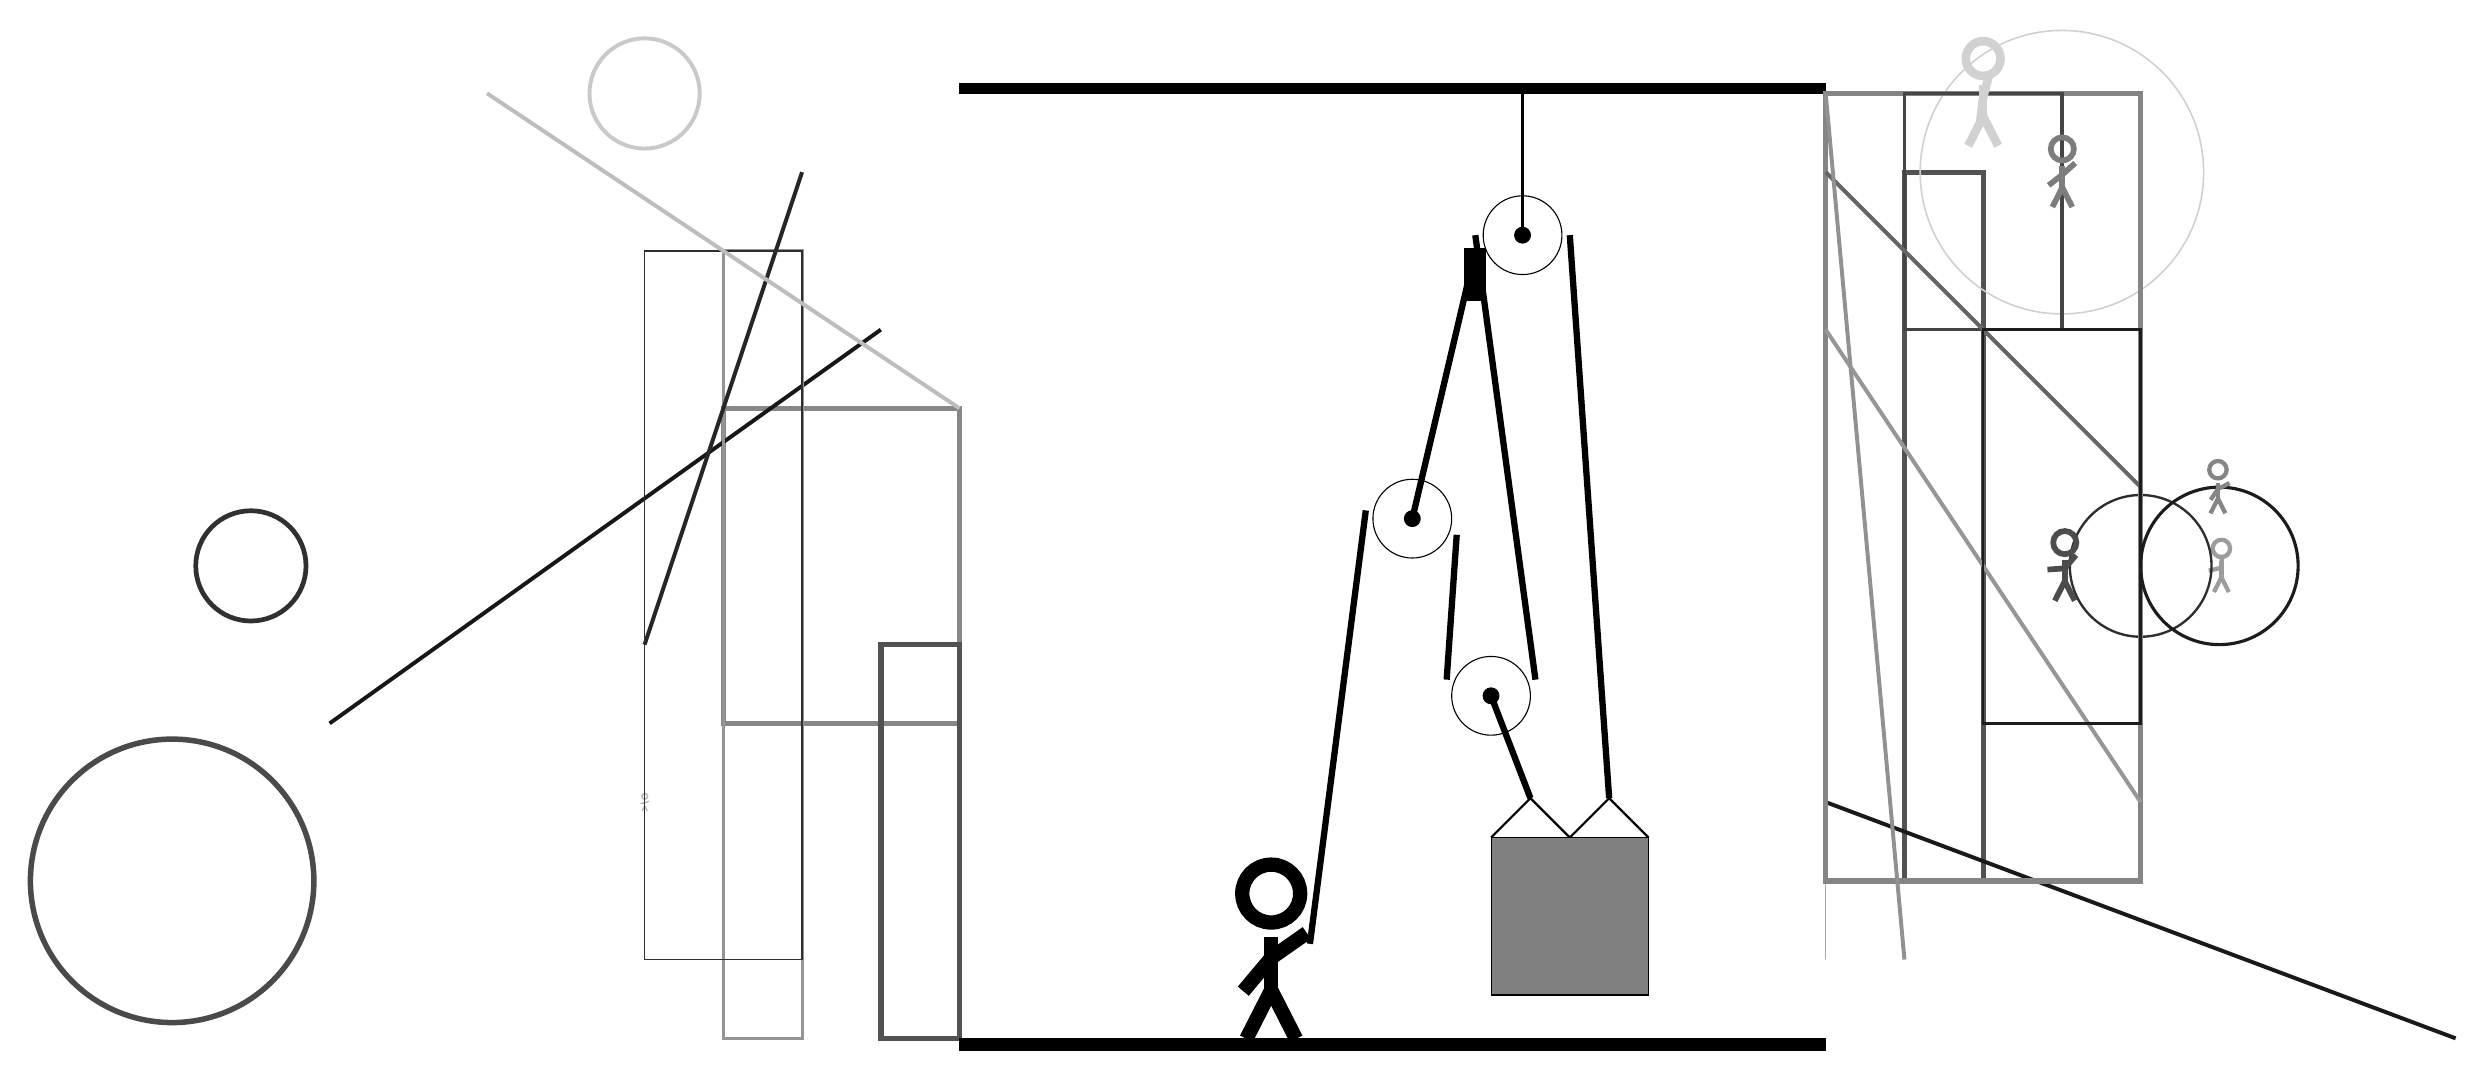
\begin{tikzpicture}
			%%%%% START %%%%%
			
			\draw[fill=black] (-6, 9) rectangle (5, 9.125);
			
			\draw (-0.25, 3.6) circle (0.5);
			\draw[fill=black] (-0.25, 3.6) circle (0.1);
			
			\draw (0.75, 1.35) circle (0.5);
			\draw[fill=black] (0.75, 1.35) circle (0.1);
			
			\draw (1.15, 7.2) circle (0.5);
			\draw[fill=black] (1.15, 7.2) circle (0.1);
			\draw[very thick] (1.15, 7.2) -- (1.15, 9);
			
			\draw[thick]  (0.75, -0.45) -- (1.25, 0.05) -- (1.75, -0.45) -- (2.25, 0.05) -- (2.75, -0.45);
			\draw[fill=black!50] (0.75, -0.45) rectangle (2.75, -2.45);
			
			\draw[line width=0.2mm, color=black!45] (7, -1) rectangle (7, 2);
			
			\draw[line width=0.6mm, color=black!68] (7, -1) rectangle (6, 8);
			\draw [line width=0.7mm, color=black!71](-16, -1) circle (1.8);
			\draw[line width=0.5mm, color=black!90](5, 0) -- (13, -3);
			
			\draw [line width=0.6mm, color=black!81](-15, 3) circle (0.7);
			
			\node[line width=0.6mm, color=black!39] at (10, 3) {\Strichmaxerl[3][13][88]};
			
			\draw [line width=0.3mm, color=black!82](9, 3) circle (0.9);
			
			\draw [line width=0.2mm, color=black!19](8, 8) circle (1.8);
			\draw[line width=0.2mm, color=black!34] (5, -2) rectangle (5, 8);
			\draw [line width=0.5mm, color=black!21](-10, 9) circle (0.7);
			
			\draw[line width=0.5mm, color=black!31](8, 5) -- (5, 8);
			
			\node[line width=0.2mm, color=black!70] at (8, 3) {\Strichmaxerl[4][4][50]};
			\draw[line width=0.7mm, color=black!47] (-6, 1) rectangle (-9, 5);
			
			\draw[line width=0.7mm, color=black!48] (5, 9) rectangle (9, -1);
			\draw[line width=0.4mm, color=black!73] (6, 6) rectangle (8, 9);
			\draw[line width=0.5mm, color=black!60](5, 8) -- (9, 4);
			
			\draw [line width=0.4mm, color=black!89](10, 3) circle (1.0);
			\draw[line width=0.5mm, color=black!43](5, 9) -- (6, -2);
			\node[line width=0.4mm, color=black!28] at (-10, 0) {\Strichmaxerl[1][12][19]};
			\node[line width=0.4mm, color=black!51] at (8, 8) {\Strichmaxerl[4][38][42]};
			\node[line width=0.7mm, color=black!48] at (10, 4) {\Strichmaxerl[3][56][27]};
			
			\draw[line width=0.5mm, color=black!41](9, 0) -- (5, 6);
			
			\draw[line width=0.5mm, color=black!91](-7, 6) -- (-14, 1);
			\draw[line width=0.4mm, color=black!42] (-8, 7) rectangle (-9, -3);
			\draw[line width=0.7mm, color=black!68] (-6, -3) rectangle (-7, 2);
			
			\draw[line width=0.3mm, color=black!89] (7, 1) rectangle (9, 6);
			
			\draw[line width=0.5mm, color=black!85](-10, 2) -- (-8, 8);
			\draw[line width=0.2mm, color=black!82] (-8, 7) rectangle (-10, -2);
			\node[line width=0.4mm, color=black!18] at (7, 9) {\Strichmaxerl[6][83][75]};
			\draw[line width=0.5mm, color=black!26](-6, 5) -- (-12, 9);
			
			\draw[line width=0.8mm] (-0.25, 3.6) -- (0.55, 7.0);
			\draw[line width=0.8mm, fill=black](0.45, 6.4) rectangle (0.65, 7.0);
			\draw[line width=0.8mm] (-1.55, -1.8) -- (-0.8409, 3.7042);
			\centerarc[line width=0.8mm](-0.25, 3.6)(-20:170:0.6);
			\draw[line width=0.8mm] (0.3138, 3.3948) -- (0.1862, 1.5552);
			\centerarc[line width=0.8mm](0.75, 1.35)(160:380:0.6);
			\draw[line width=0.8mm] (1.3138, 1.5552) -- (0.55, 7.2);
			\draw[line width=0.8mm](0.75, 1.35) -- (1.25, 0.05);
			\centerarc[line width=0.8mm](1.15, 7.2)(0:180:0.6);
			\draw[line width=0.8mm] (1.75, 7.2) -- (2.25, 0.05);
			
			\node at (-2, -1.9) {\Strichmaxerl[10][50][35]};
			
			\draw[fill=black] (-6, -3) rectangle (5, -3.15);
			
			%%%%% END %%%%%
		\end{tikzpicture}
	\end{figure}	
\end{document}